\chapter{General State of the Art}


\section{Context}

To replace materials that are very practical but very problematic for our environment, convince people of the usefulness of the replacement. on the one hand, by making functional objects. But also by opening the door to new imaginations that broaden the scope of what's possible. that's why, in the same way as classical research, design helps to shape this problem. 
\begin{marginfigure}[-5cm] % Adjust the vertical placement
    \centering
    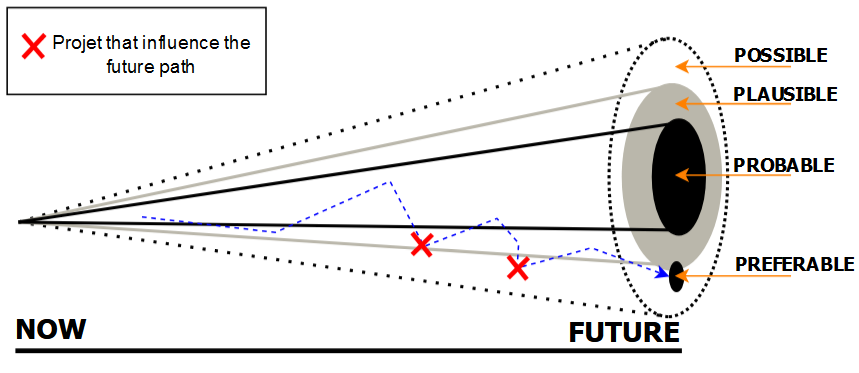
\includegraphics[width=\linewidth]{images/futures_cone2.png}
    \caption{futures cone representation}
    \label{fig:futures code}
\end{marginfigure}
Science in this field relatively new. The starting point differs depending on how define biomaterials and how make, or rather grow them. 
More globally, biomaterials are at the crossroads of many fields of scientific and even artistic research. From agriculture to design, from synthetic biology to fashion, from DIY fermented drink to biohacking in the kintchen\cite{CiteTheOdin}.
This is in line with new interdisciplinary courses integrating biodesign, such as MIT's "How To Grow (Almost) Anything" course\cite{CiteMITHTGAA}. 

As matter of fact, the starting point might be the first crops domestication. At this time the goal was only to produce food, and the process were optimized by selective breeding. By taking the plants with the biggest fruit or the best resistance to environment, from generation to generation plants were "optimized" for the population.
Besides, the use of wood are very use in numerous sectors\cite{ramage2017wood} push by international directive of less CO2 emmission and waste. 
  
However, today, biomaterials or biobased materials in this study are more in line with the aim of replace existing materials like plastics.
This biomaterials production projects are aimed to create in the futures of cone plausible or possible futures. 
Moreover the development of this new materials go hand in hand with the evolution of new machines for biomaterials. Bioreactors are controlled environment systems. There is no notable differences in hardware part from bioreactors in the litterature. The general form is a isolated space from outside environmental conditions, 
combine with a controler responsible of sensors and actuator (i.e :fogger, fan, thermal resistance...). The controler is also responsible to send data when monitoring is wanted. All powered by energy from different sources. 

Multiple reviews\cite{cottet2020biobased}\cite{vinod2020renewable}\cite{hairon2022bio} about biobased materials support for the fact that today's synthetic materials, especially those derived from oil, are a problem for human and ecosystem health.
These studies reveals the strong interess of these materials in term of sustainability and low cost production, and "by reducing wastages, landfills
and toxic emissions leading to greener and cleaner environment". They also show end proprieties these materials are distinguished by their biodegradability and compostability. Which also makes them interesting for their end-of-life properties. 
However, there are concers about a lack of large scale industrialisation and a lack standadise methodology \cite{andrew2022sustainable}. This leads to a lack of confidence in mechanical properties, as the absence of standardization, give rise to the limited exploitation of technical data on characteristics such as tensile strength, compression, fatigue, impact resistance and flammability, makes assessment more difficult.   
Into the bargain, most of these materials are and highly anisotropic.

\paragraph[short]{Industry} 
Ecovative and MycoWorks lead in mycelium-based biomaterials. Ecovative creates eco-friendly alternatives to plastics for packaging and construction, while MycoWorks focuses on sustainable mycelium leather, targeting fashion and luxury markets.
\paragraph[short]{In Design} 
Suzanne Lee, through Biofabricate, pioneers biofabrication in design, using biological processes to grow sustainable materials like microbial leather, pushing the boundaries of traditional manufacturing and eco-conscious design.


\section{Biomaterial}
text def biobased biomaterial biofabricated biosynthetic;;;;;;;;;;;;;;;;;;;;;;;;;;;;;;

\subsection{S.C.O.B.Y Lether} 
% \begin{marginfigure}
%     \centering
%     \includegraphics{images/.png}    
%     \caption{}
%     \label{fig:}
% \end{marginfigure}
\paragraph[short]{Definition } 
S.C.O.B.Y, aim to Symbiotic Culture Of Bacteria and Yeast, during this symbiotic culture a lot of biochimical element are tranformed or exchanged by bacteria and yeast.
Among this biochimical elements, there is bacterial cellulose. Bacterial cellulose (BC) is a biopolymer that grows on the surface of the culture medium. which, once dry, produces a biomaterial with the appearance of leather. 

\begin{marginfigure}
    \centering
    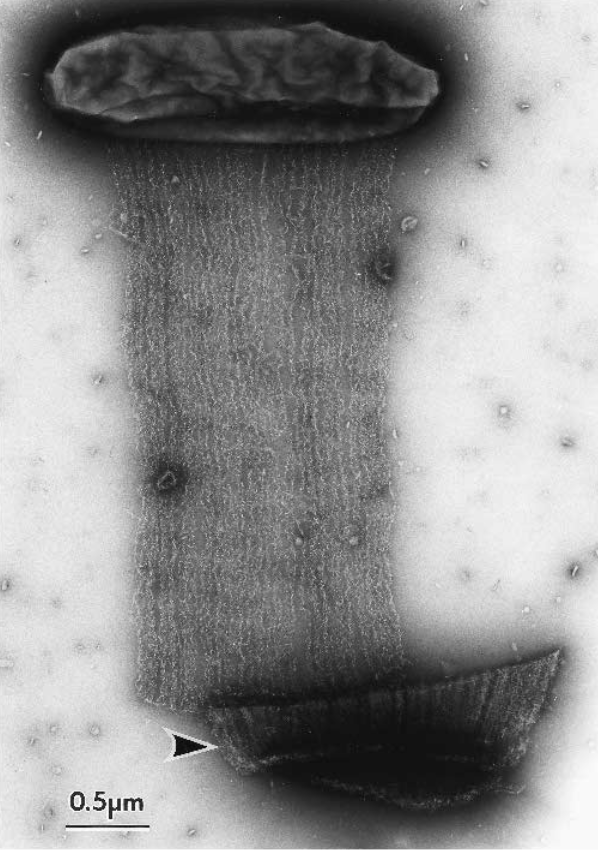
\includegraphics{images/bacteriaandcellulose.png}
    \caption{Negatively stained coarse band-like cellulose assembly produced during 6 h of incubation at 4 °C. At the bottom of the figure, a
    detached dense assembly of cellulose is also observed (indicated by the arrowhead)from\cite{hirai2002tem}}
    \label{fig:bacteriaandcellulose}
\end{marginfigure}

More precisely, 2 metabolic processes are at play, in a kind of “double” fermentation. 
on the one hand, alcoholic fermentation by yeasts. In other words, the glucoses will be converted into ehtanol. 
On the other hand, “acetic fermentation” by bacteria. In other words, the ethanol will be converted into acetic acid. see \ref{fig:fermentation formula} and \ref{fig:metabolic}

% C_6H_{12}O_6 + 2 \, \text{ADP} + 2 \, P_i \rightarrow 2 \, \text{ATP} + 2 \, H_2O + 2 \, \textcolor{red}{CH_3CH_2OH} + 2 \, CO_2

% \textcolor{red}{CH_3CH_2OH} + O_2 \rightarrow CH_3COOH + H_2O
\begin{figure}[h]
    \centering
    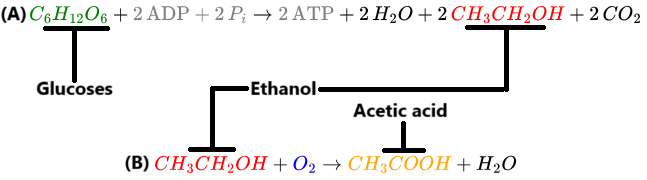
\includegraphics{images/formule-chimique.png}
    \caption{fermentation formulas, (A) : Alcoholic fermentation, (B) : Acetic fermentation}
    \label{fig:fermentation formula}
\end{figure}

\begin{figure}[h]
    \centering
    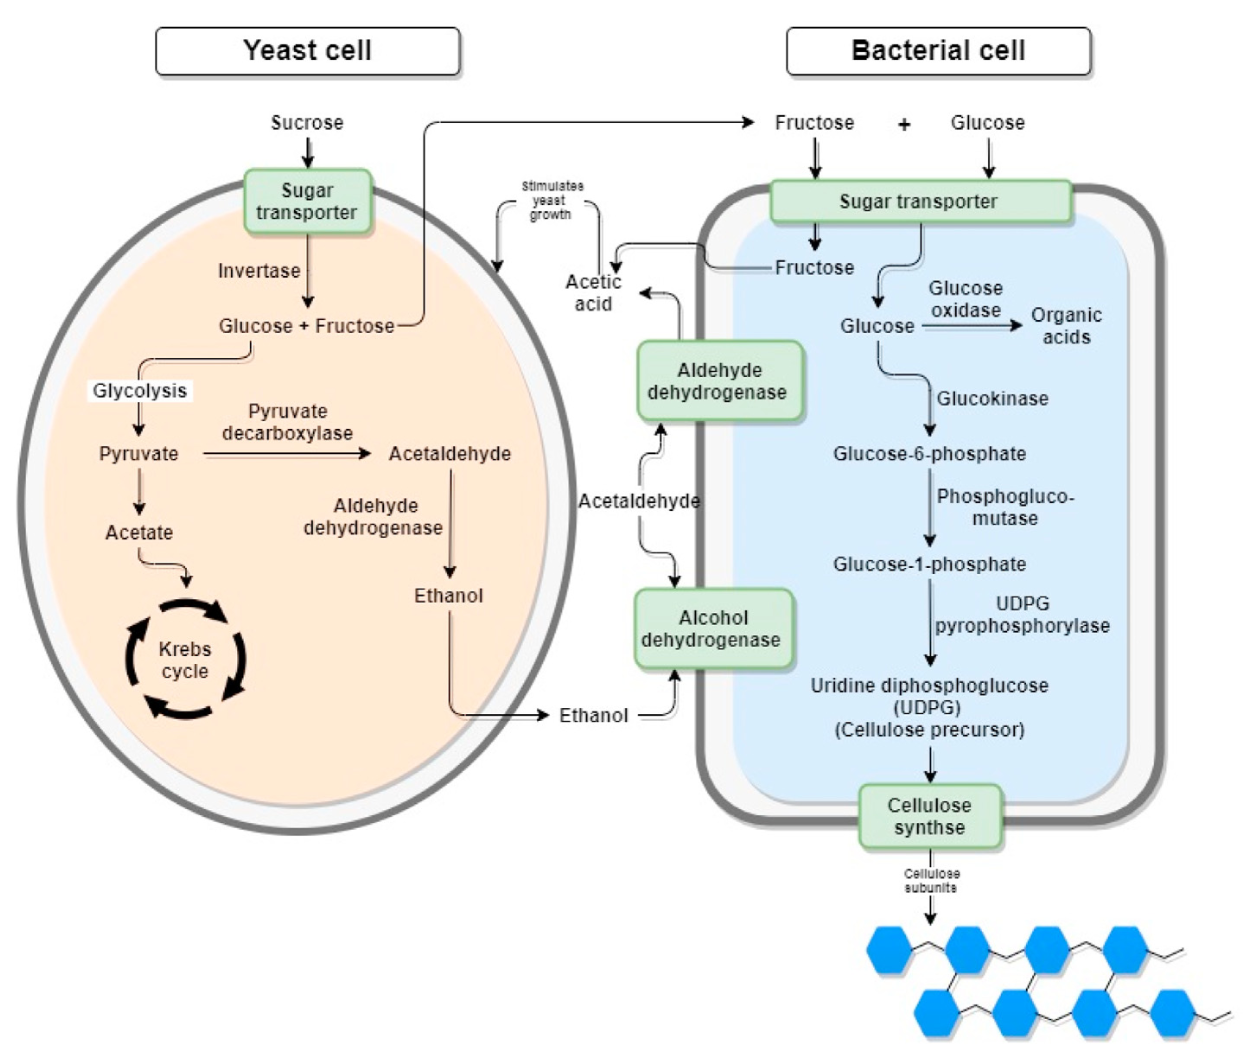
\includegraphics{images/schema_metabolique.png}
    \caption{Metabolism of substrates by the symbiotic culture of bacteria and yeast from\cite{laavanya2021current}}
    \label{fig:metabolic}
\end{figure}

In addition to the metabolic processes that allow these microorganisms to survive and reproduce, bacteria will also synthesize this so-called bacterial cellulose.\ref{fig:bacteriaandcellulose} 
More popularly, scoby is the culture used to make fermented tea-based drinks called kombucha. 
To grow cellulose, the recipe is similar: a strain of scoby, water, sugar and vinegar. The difference is that it is preferable first to select the strains that produce the most cellulose. 

Another element that emerges from the literature, without taking bioreactors into account, is that cellulose production decreases more and more over time and follows a kind of inverse exponential curve tending towards a finite value that corresponds to the maximum value of cellulose produced.\cite{chong2024modelling}.
as pictured \ref{biomasse-cellulose-grap}. There are two reasons why cellulose production stops: firstly, of course, because there is less and less nutrient in the culture medium; secondly, because the production of cellulose on the surface will eventually self-isolate the culture medium; and thirdly, as seen in equation (B) in \ref{fig:fermentation formula}, oxygen is important for bacterial fermentation, and therefore for their survival and development. 
\begin{marginfigure}
    \centering
    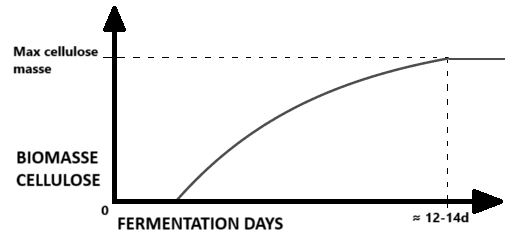
\includegraphics{images/biomasse-cellulose.png}
    \caption{model curve for cellulose biomasse over time}
    \label{fig:biomasse-cellulose-graph}
\end{marginfigure}

so, to sum up, in order to have good cellulose production, you need to maintain fermentation for the proper development of bacteria and yeast. at the same time, you need to make sure that the medium doesn't auto-asphyxiate.



\paragraph[short]{Use}

Roussel et al.'s extensive mapping\cite{roussel2023processes} effectively illustrates the diverse ecosystem around SCOBY leather production, showing Bacterial Cellulose (BC) is divided across varied fields: biology, medicine, food, textiles, and materials science. This broad range of applications reveals substantial potential, though these fields are rarely interconnected and often operate independently.
even if some of these applications are speculative or artistic, they tell us how a discipline approaches the problem of growth, and what the advantages and disadvantages of a particular approach are. Furthermore, it's interesting to note that a combined approach could give rise to projects with a strong impact on their dicipline. for example, between the industrial and medical machine clusters. 
\begin{figure}
    \centering
    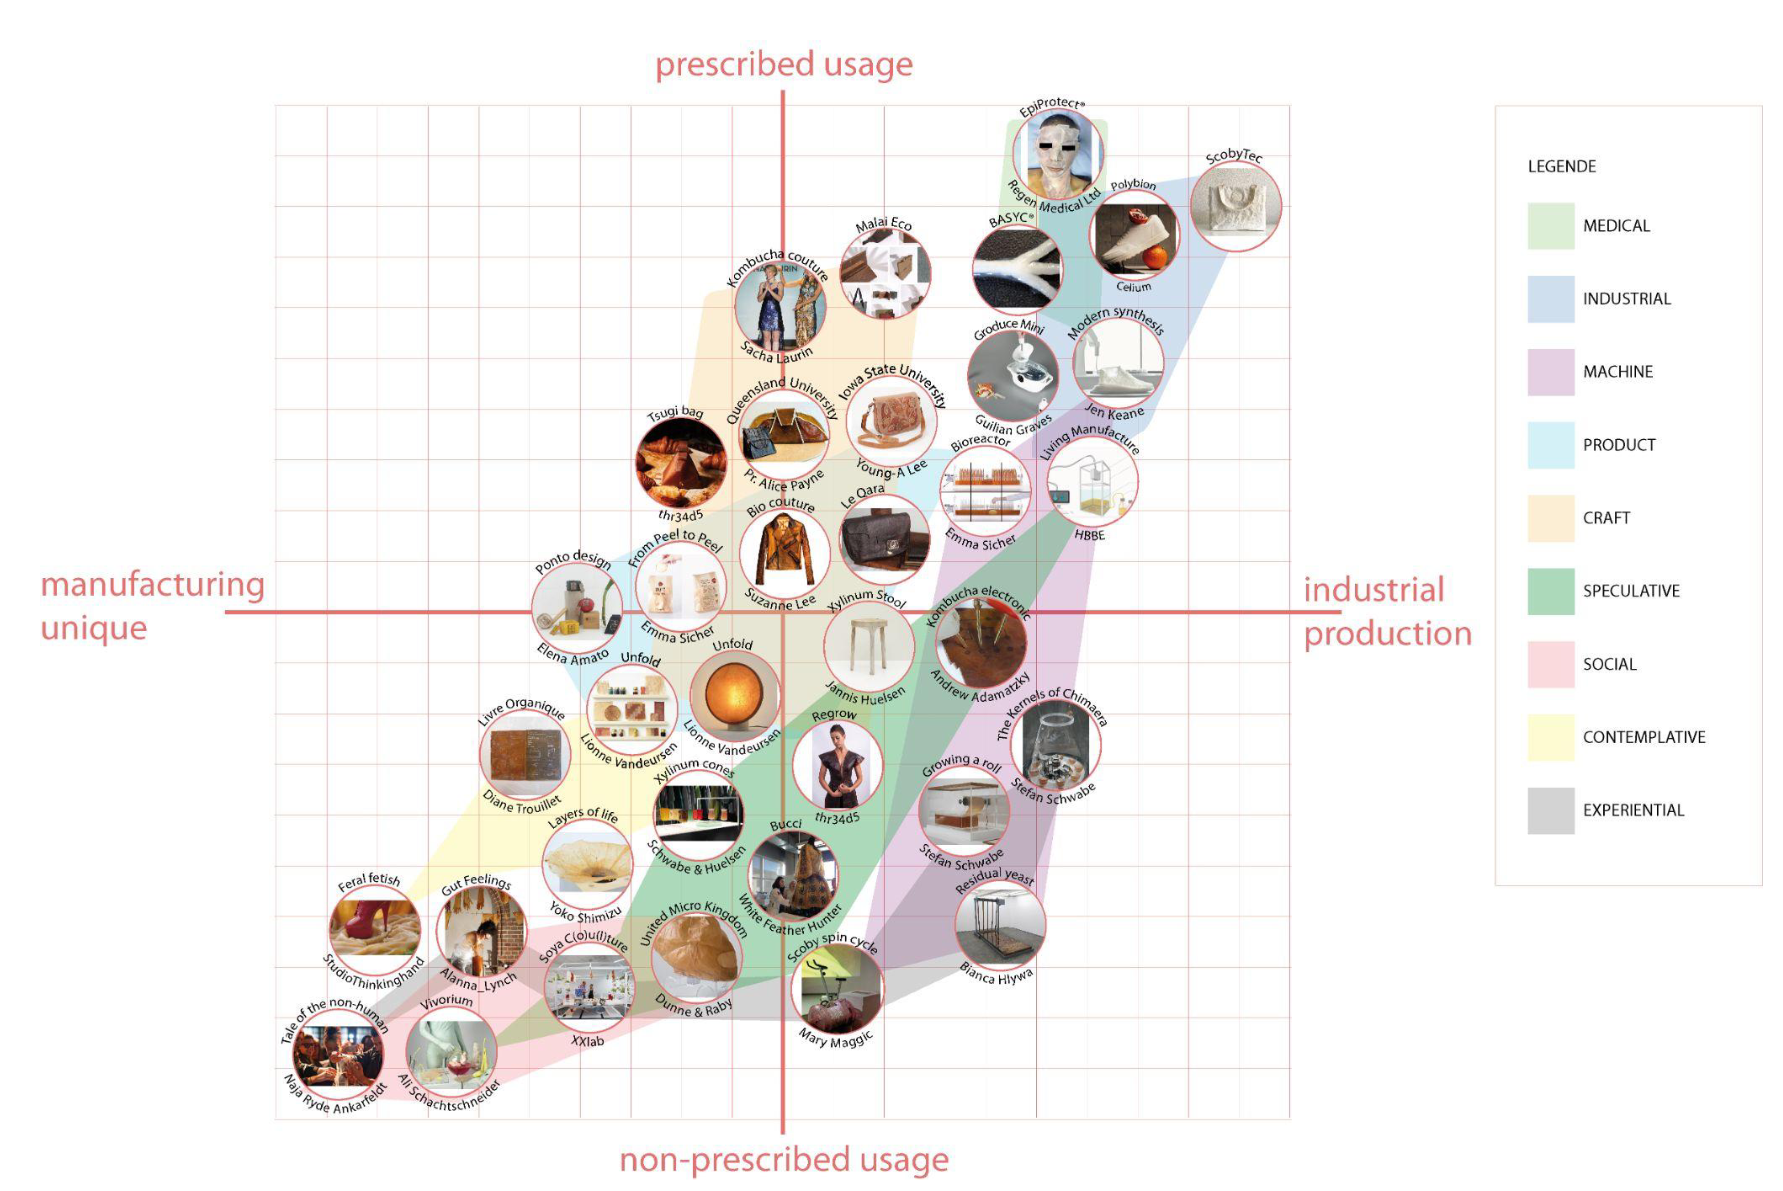
\includegraphics[width=1.4\textwidth]{images/mapping-practices-kombu.png} % Adjust width to 80% of text width
    \caption{Processes, Fabrication and Design with Kombucha Bacterial Cellulose: Mapping Practices from\cite{roussel2023processes}}
    \label{fig:graph-vivien}
\end{figure}




The work of zang et al\cite{zang2015investigation} describes how Bacterial cellulose (BC) exhibits exceptional biocompatibility, making it a promising material for various biomedical applications, particularly in vascular tissue engineering. Several studies have demonstrated that BC does not induce significant clotting or hemolysis when in contact with blood, indicating its favorable interactions with the bloodstream. This property is critical for any material intended for use in vascular implants or scaffolds, as it reduces the risk of thrombosis and ensures that blood flow is maintained without complications.
One of the earliest and most significant direct applications of bacterial cellulose (BC) membranes in the biomedical field is their use in wound dressings. 

Fontana et al. (1990)\cite{fontana1990acetobacter} were among the first to describe the use of BC as a substitute for burned skin. Since their pioneering work, the literature has seen a growing number of studies focused on wound dressing applications. Cellulose-based dressings are now widely recommended as a temporary solution for treating various types of wounds.\cite{de2016multipurpose} 
The cultivation techniques seem to be very classic in the future of microorganism cultivation. with classic laboratory equipment. however, in the recipes, the use of tea is hardly or not at all mentioned “The strain being used is a wild type microorganism isolated from a
decomposing homemade Matricaria sp. infusion”\cite{fontana1990acetobacter}. the quantities produced are deliberately small. but also the peridoe of growth is very reduced. 

\begin{marginfigure}
    \centering
    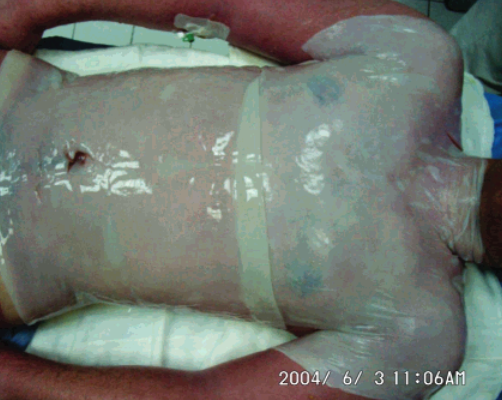
\includegraphics{images/medical_appl.png}    
    \caption{illustation BC use in medical applications from \cite{czaja2007future}}
    \label{fig:medical applications}
\end{marginfigure}

otherwise, from a more aesthetic point of view, jen keane's work on “this is grow".Materials designer and creative researcher Jen Keane developed her project “This is Grown” during her Master’s degree at Central Saint Martins, driven by her frustration with plastics.Blending design, science, technology, and craft, Keane is inspired by sustainability and intrigued by new digital and biological tools. In this project, she created a shoe upper grown as a single piece, using continuous yarn held together by cellulose produced by Komagataeibacter rhaeticus bacteria. This innovative, organism-driven approach enabled her to manipulate the growth process for a technique called "microbial weaving." 
The resulting hybrid material leverages the natural properties of bacterial cellulose, producing a strong, lightweight product with minimal waste. By employing a traditional weaving-like method where the warp is woven by Keane and the bacteria grow the weft at the nanoscale, the technique allows for intricate patterns and enhanced material strength in multiple directions.

In a similar vein to Jen Keane's work, Suzanne Lee, also associated with Central Saint Martins, pioneered the concept of BioCouture—a movement exploring DIY and traditional techniques for growing materials. Lee’s work has served as a foundational "nursery" of ideas for biodesign, integrating biology into fashion. By cultivating Komagataeibacter bacteria in a nutrient-rich solution, Lee was able to produce bacterial cellulose sheets that could be treated and crafted into wearable garments.

\begin{marginfigure}
    \centering
    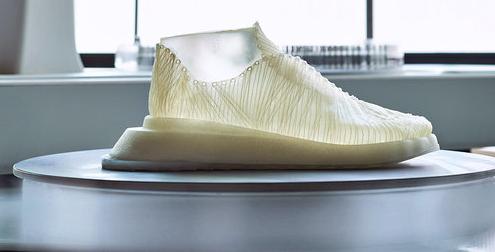
\includegraphics{images/jen_keane.png}
    \caption{Jen Keane - this is grow}
    \label{fig:jen_keane}
\end{marginfigure}

\begin{marginfigure}
    \centering
    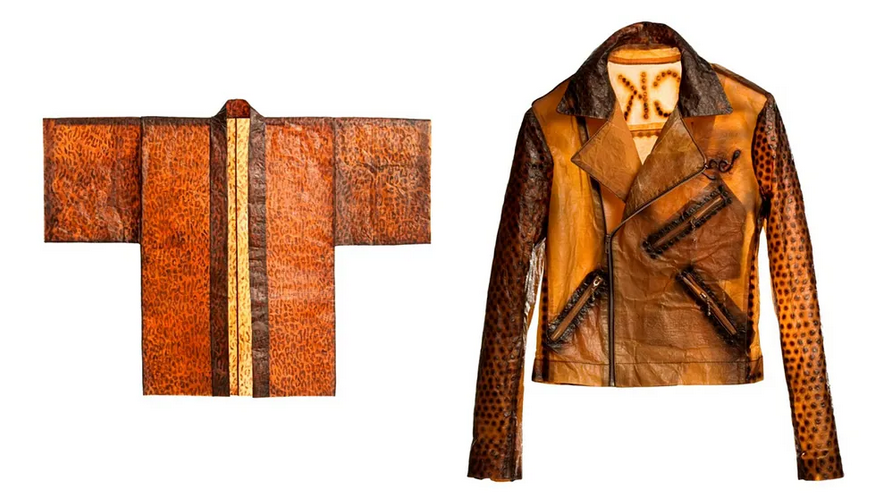
\includegraphics{images/suzanne_lee.png}
    \caption{Suzanne Lee - BioCouture}
    \label{fig:Suzanne Lee}
\end{marginfigure}

%\cite{caro2021bacterial}

Nicolae et Al. propose an framework \cite{nicolae2023biohybrid} of how build biohybride devince that incorporates electronics. 
Furthermore, they discuss the development of biohybride devine in HCI. The framework describe how prototyping with Bacterial cellulose. It distint three phase of BC life cycle where prototyping : Growth, Stabilization and Inanimate. 
The growth phase is mostly the part where add embed electronics or other particular material like textile. (This thesis will later discuss how the bioreactor can influence the material itself on this phase.)
The Stabilization phase is just after the growth phase before the biomaterial is dry. This phase enable 3D forming as the material is more maleable then after dry process. This phase was the phase use in medical applications for wound dressing, as the bacterial cellulose is still wet. the project this is grow by Jen keane might be between this two first phase.
The inanimate phase corresponds to the more traditional phase, after dry, where biomaterials resemble textile leather, and it's this part that Suzanne Lee focuses on in her biocouture project. 

\begin{figure}[h]
    \centering
    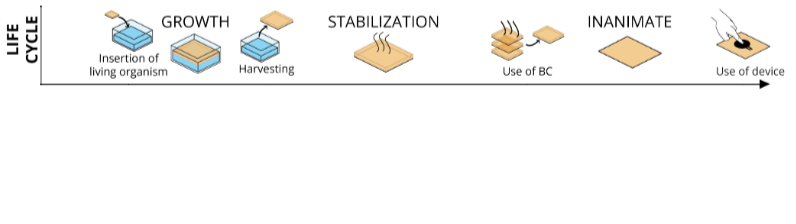
\includegraphics[width=1.4\textwidth]{images/phase-proto.png}
    \caption{BC life cycle phases as material from\cite{nicolae2023biohybrid}}
    \label{fig:life cycle}
\end{figure}




\subsection{Mycelium material}

% \begin{marginfigure}
%     \centering
%     \includegraphics{images/.png}    
%     \caption{}
%     \label{fig:}
% \end{marginfigure}


\paragraph[short]{Definition}
"Mycelium is a root-like structure of a fungus consisting of a mass of branching, thread-like [called] hyphae."\cite{wikipediaMycelium}. Actually, The visible part of a mushroom during a forest walk is merely its surface structure. In the common sense, " mushroom " only refers to the fruiting bodie part,the reproductive part. 
On the other hand, Mycelium material, Mycomaterial, or mycelium-based biocomsites etc. Is a biofabricated material like bacterial cellulose. the general principle is to mix mycelium with an organic substrate. as in nature, the mycelium will secrete enzymes that dissolve its food, but also bond\cite{MonikaBrandićLipińskaHBBE} (\ref{fig:myco-bond}) and aglomarate the substate at cellular scale. 
Thus, we can give a shape to the inoculated substate and after the mycelium grow in all the substate like cellulose, it will be dry to give biocomposite. During these processes the substrate can be molded into various shapes to change the form of the biocomposite. 

\begin{marginfigure}
    \centering
    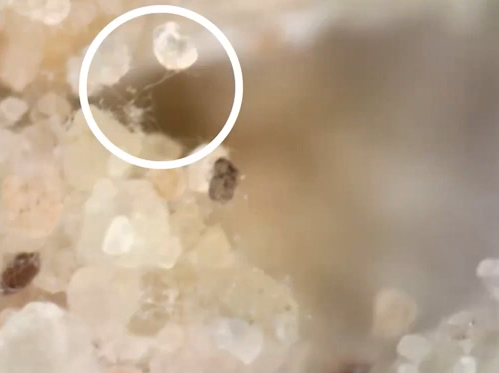
\includegraphics{images/bond-mycelium.png}    
    \caption{Mycelium at micro level on biocomposite from  Monika Brandić Lipińska | Space to Grow - Design of Biological Construction of Living Habitation on Mars}
    \label{fig:myco-bond}
\end{marginfigure}

A review of 2023,\cite{alaneme2023mycelium} show that Mycelium based composites, show that \ref{trend} the publication grew in the field.
This review also illustrates witch muchroom mycelium is use to build mycelium-base biocomposite, not all mushroom mycelia have the same characteristics, and some will produce harder or softer materials. on the other hand, the choice of substrate and the mass in which it is inoculated will also have an impact on the mechanical characteristics. furthermore, as the choice of mycelium itself influences how the mycelium will grow in the substrate, (a mycelium more adapted to a substrate with wood lignin for example will grow better in a substrate with wood lignin) some substrates give better results depending on the species of mushroom. 
however, it would seem that it is above all the choice of substrate that influences the mechanical properties, independently of the mycelium chosen.  

\begin{marginfigure}
    \centering
    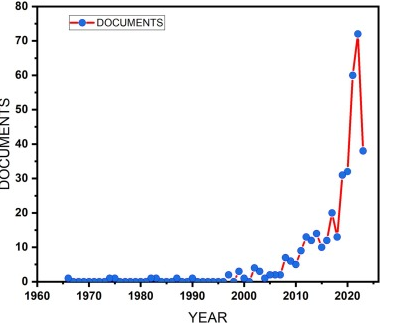
\includegraphics{images/publication on mycelium-based.png}    
    \caption{Trend of scientific publication on mycelium-based composites from 1966 to 2023 from \cite{alaneme2023mycelium}}
    \label{fig:trend}
\end{marginfigure}

Research by Elsacker et al.\cite{elsacker2019mechanical} and Yang et al.\cite{yang2017physical} demonstrates that the design of the substrate mold significantly influences the mechanical properties—such as compressive strength, stiffness, and Young’s modulus—of mycelium-based composites (MBCs). Mold shape, density, and stiffness play a crucial role as the inoculated mix of mycelium and substrate fills the mold, impacting the final density and fiber orientation of the MBCs. Various packing methods, including polyethylene and porous bags, PVC, and thermo-formed plastic molds, are employed, with each method affecting the quality and structure of the fungal skin. Optimal mold design remains a key area for further research to improve MBC production.

Reports indicate that the low thermal conductivity, high acoustic absorption, and fire-resistant qualities of MBCs have made them highly suitable for use in building and construction. \cite{ghazvinian2019mycelium}

\paragraph{Use}

There is no mapping practice of mycelium in the litterature like Roussel et al.'s \cite{roussel2023processes} did for SCOBY. but we believe that the mycelium shares similarities with the interdisciplinary clustering parameters presented.
Mycelium-based biocomsites have been uses both in the speculative and industrial sectors as well as in research.

\begin{figure}[h]
    \centering
    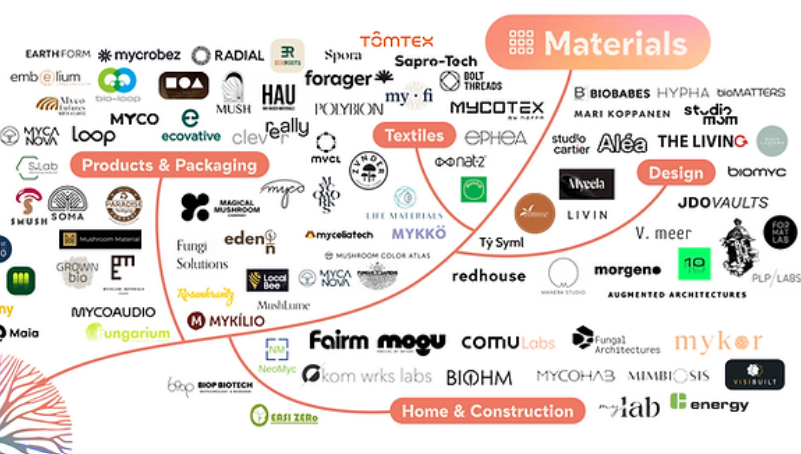
\includegraphics{images/mycelium-indus-tree.png}
    \caption{materials field industry for Mycelium composite}
    \label{fig:indus-tree}
\end{figure}

The mapping of Mycostory, illustrates (a bit) different scector in Mycelium materials industry. design practice aside, there are 3 main ways in which MBC tends to be used functionally: packaging, construction, and textiles. 
it's mainly packaging and construction that are similar to biocomposite techniques. the textile sector is full of other methods for making mycelium leather that differ from mycelium-based composites. 


Ecovative is a pioneer in this field, particularly in packaging, where their products demonstrate how mycelium-based composites (MBCs) can replace traditional, environmentally harmful materials like Styrofoam. By using agricultural waste combined with mycelium, Ecovative creates biodegradable packaging that performs similarly to synthetic foams, offering both protective qualities and a fully compostable lifecycle. they've managed to scale up the techniques we've developed before so that they can supply other companies with products in large quantities. 
\begin{figure}[h]
    \centering
    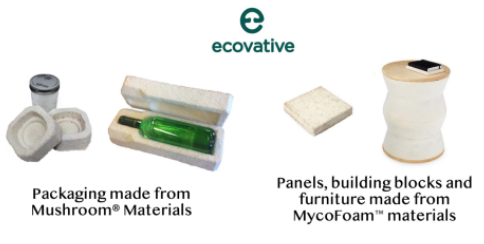
\includegraphics{images/ecovative.png}
    \caption{}
    \label{fig:ecovative}
\end{figure} 

The works of Monika Brandić Lipińska and NIAC (NASA innovative advanced concept) suggests the use of mycelium\cite{rothschild2019myco} to build on mars mycelium structures\cite{brandic2022biological}.

The works of Monika Brandić Lipińska and NASA’s Innovative Advanced Concepts (NIAC) propose utilizing mycelium as a sustainable and adaptable material for constructing habitats on Mars. Rothschild et al. (2019) \cite{rothschild2019myco} in their NIAC report suggest that mycelium-based structures could be grown on-site using local Martian resources, reducing the logistical challenges and costs associated with transporting building materials from Earth’s adaptability and self-repair potential, combined with its low resource requirements, make it a promising candidate for developing structures in the harsh Martian environment.

Brandić Lipińska’s research\cite{brandic2022biological} further explores how biological materials like mycelium could be integrated into extraterrestrial construction. Her work emphasizes the environmental and structural benefits of mycelium, such as thermal insulation, radiation shielding, and the potential to grow complex architectures with minimal human intervention. By incorporating mycelium into Martian habitat designs, these studies pave the way for innovative construction techniques that leverage living organisms to create adaptable, eco-friendly, and self-sustaining habitats in space .







\subsection{Other Biomaterial}




















\section{Bioreactor \& Controlled Environment }

\subsection{Controlled Environment} 



















\subsection{Bioreactor}
\subsection{Bioreactor S.C.O.B.Y}
\subsection{Bioreactor Mycelium}



\section{Discution and limitation}